\documentclass[11pt]{article}
\usepackage[margin=1in]{geometry}
\usepackage{booktabs}
\usepackage{graphicx}
\usepackage{amsmath}
\usepackage{amssymb}
\usepackage{microtype}

\title{Fine-mapped single-cell eQTL evaluation of AlphaGenome fine-tuning}
\author{}
\date{}

\begin{document}
\maketitle

\section{Overview}
We evaluate whether sequence-derived mutation effects distinguish fine-mapped
single-cell expression quantitative trait loci (eQTLs). A positive is a
variant with posterior inclusion probability (PIP) greater than $0.75$ and a
negative is a variant with PIP less than $0.01$. The evaluation uses human
fine-mapping panels and a $1\,\mathrm{Mb}$ sequence window centered on the
transcription start site (TSS) of the associated gene.

The primary comparison is a trained head-only model versus the two best
available joint fine-tuned models, a LoRA model and a LoRA+LoCon model. The
benchmark retains
up to 1,000 variants in each PIP class per fine-mapping panel with a fixed
random seed. The raw and retained counts are recorded with the benchmark
output.

\section{Cell-type matching}
The 35 fine-mapping panels use the prefixes Ast, End, Ext, IN, MG, OD, and OPC,
with numbered panels denoting subpanels. The trained head-only, LoRA, and
LoRA+LoCon models use the same target track definitions. The matching used for
these models is shown below. A separate native AlphaGenome analysis evaluates
all valid pretrained RNA-seq and CAGE tracks, without adding a newly initialized
head.

\begin{table}[ht]
\centering
\small
\caption{Fine-mapping panel to RNA-track matching for the trained head-only,
LoRA, and LoRA+LoCon models. A numbered panel inherits the mapping for its
prefix.}
\label{tab:cell_matching}
\begin{tabular}{@{}p{0.16\linewidth}p{0.37\linewidth}p{0.37\linewidth}@{}}
\toprule
Panel prefix & Trained head-only & LoRA and LoCon \\
\midrule
\texttt{Ast*} & ASC & ASC \\
\texttt{End*} & Endo & Endo \\
\texttt{Ext*} & Mean of L2/3 IT, L4/5 IT, L5/6 NP, L5 ET, L5 IT, L6 CT, L6 IT CAR3, and L6b & Same \\
\texttt{IN*} & Mean of LAMP5, PVALB, SNCG, SST, and VIP & Same \\
\texttt{MG*} & MGC & MGC \\
\texttt{OD*} & ODC & ODC \\
\texttt{OPC*} & OPC & OPC \\
\bottomrule
\end{tabular}
\end{table}

The panel labels do not exactly match the available pretrained output tracks.
The native model therefore receives a separate track-level analysis; it is not
represented by the trained-head comparison above.

\section{Mutation effects}
For variant $i$, let $\mathbf{y}_{i,r}\in\mathbb{R}^{B\times C}$ and
$\mathbf{y}_{i,a}\in\mathbb{R}^{B\times C}$ be the reference and alternate
RNA predictions at the model's 128 bp resolution, where $B$ is the number of
output bins and $C=19$ is the number of RNA tracks. Let $\mathcal{C}_g$ be the
track indices for the matched cell group. The TSS score is
\begin{equation}
s_i^{\mathrm{TSS}}=\frac{1}{|\mathcal{C}_g|}\sum_{c\in\mathcal{C}_g}\left|y_{i,a,b_{\mathrm{TSS}},c}-y_{i,r,b_{\mathrm{TSS}},c}\right|,
\end{equation}
where $b_{\mathrm{TSS}}$ is the 128 bp bin containing the TSS. The gene score
is the corresponding mean absolute alternate-reference difference after
averaging each track over all 128 bp bins overlapping the annotated gene
span,
\begin{equation}
s_i^{\mathrm{gene}}=\frac{1}{|\mathcal{C}_g|}\sum_{c\in\mathcal{C}_g}\left|\frac{1}{|\mathcal{B}_i|}\sum_{b\in\mathcal{B}_i}y_{i,a,b,c}-\frac{1}{|\mathcal{B}_i|}\sum_{b\in\mathcal{B}_i}y_{i,r,b,c}\right|,
\end{equation}
where $\mathcal{B}_i$ is the set of bins overlapping the gene span. Both
scores are nonnegative because fine-mapping identifies variant probability,
not the direction of expression change. Performance is measured by AUROC
and average precision, overall and within bins of $|\mathrm{variant}-\mathrm{TSS}|$.

\section{Results}
The completed benchmark is summarized by distance from the TSS in the
following figures. The underlying per-bin AUROC, AUPR, and class counts remain
available in the machine-readable summary output.

\begin{figure}[ht]
\centering
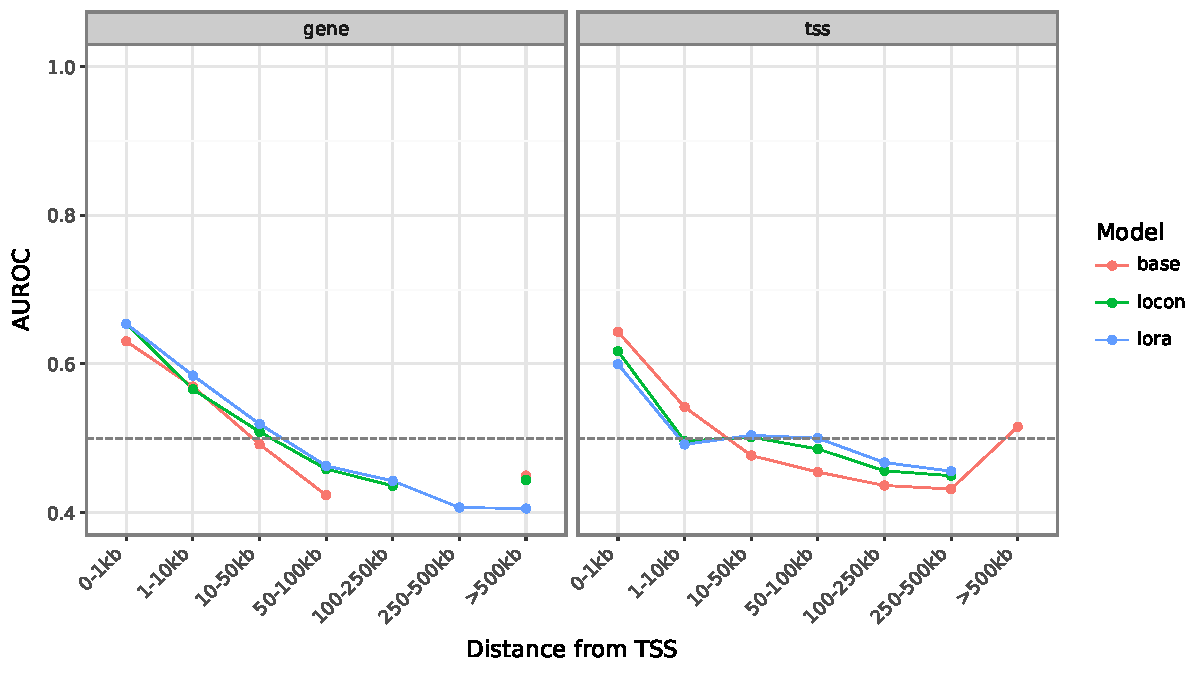
\includegraphics[width=0.95\linewidth]{figures/eqtl_auroc_by_distance.pdf}
\caption{AUROC by distance from the TSS for TSS-bin and gene-span mutation
effects. The dashed line is chance performance.}
\label{fig:eqtl_distance}
\end{figure}

\begin{figure}[ht]
\centering
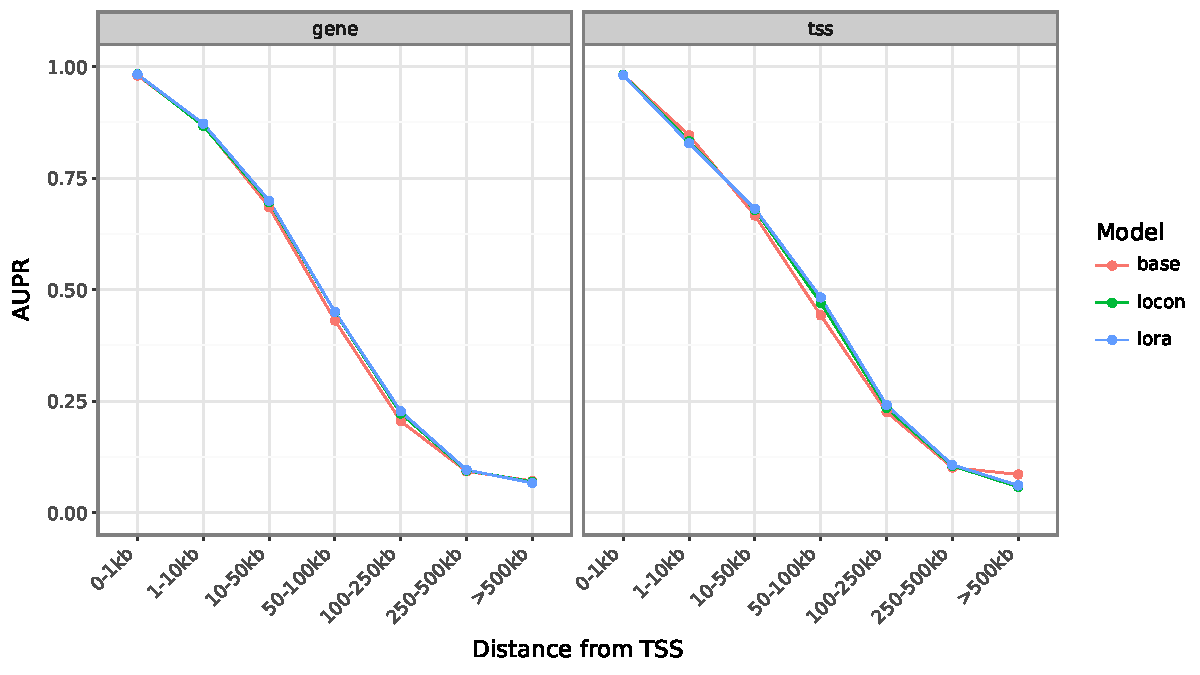
\includegraphics[width=0.95\linewidth]{figures/eqtl_aupr_by_distance.pdf}
\caption{AUPR by distance from the TSS for TSS-bin and gene-span mutation
effects.}
\label{fig:eqtl_aupr_distance}
\end{figure}

\section{Implementation details}
Fine-mapping tables are streamed from compressed PIP files. Variant alleles
are checked against the reference genome before constructing the alternate
one-hot sequence. The same reference and alternate sequences are evaluated
for every model. The head-only checkpoint was trained on the target tracks
without LoRA or LoCon adapters; the fine-tuned models retain trained heads and
adapters. All model prediction calls use the custom forward path so the
fine-tuned heads, rather than the delegated pretrained variant scorer, are
evaluated. Native AlphaGenome VEPs use the original model's valid RNA-seq and
CAGE tracks, with predictions reduced on device to the TSS bin and gene span
before signed alternate-minus-reference effects are stored. CD14-positive
monocytes are treated as a proxy for microglia. CAGE includes an
oligodendrocyte-precursor track, but the native RNA-seq panel does not contain a
direct oligodendrocyte track; this distinction is retained in cell-specificity
interpretation.

\end{document}
